%%%%%%%%%%%%%%%%%%%%%%%%%%%%%%%%%%%%%%%%%%%%%%
% Header
\documentclass[11pt]{report}
\usepackage[english]{babel}
\usepackage[utf8x]{inputenc}
\PassOptionsToPackage{hyphens}{url}\usepackage{hyperref}
\usepackage{graphicx}
\usepackage{fullpage}
\usepackage{nicefrac}
\usepackage[lastexercise]{exercise}
\usepackage[dvipsnames]{xcolor}
\usepackage{listings}
\usepackage{enumitem}
\graphicspath{ {./weekly_content/img/} }

\setlength{\parindent}{0cm}

\renewcommand{\ExerciseHeader}{\large\textbf{\ExerciseName~\ExerciseHeaderNB} - \textbf{\ExerciseTitle}\medskip}

\renewcommand{\ExePartHeader}{\medskip\textbf{\ExePartName\ExePartHeaderNB\ExePartHeaderTitle\medskip}}

\begin{document}
%%%%%%%%%%%%%%%%%%%%%%%%%%%%%%%%%%%%%%%%%%%%%%
\title{Exercises -- Week 2: \\Control Structures: Conditional Statements}
\subsubsection*{EMAT10007 -- Introduction to Computer Programming}
\subsection*{\Large Exercises -- Week 2: \\Control Structures: Conditional Statements}

\noindent\fbox{%
    \parbox{\textwidth}{%
        \subsection*{Getting Started: How to open software}
        \subsubsection*{PyCharm IDE (Integrated Development Environment)}
        \begin{itemize}
            \item{Open PyCharm on a Linux lab computer}
            \begin{itemize}
                \item{Click on Activities in the top left corner of the screen.}
                \item{Open 'Terminal' from the menu tab.}
            \end{itemize}
            \item{To instead install PyCharm on your personal computer}
            \begin{itemize}
                \item{Click on Activities in the top left corner of the screen.}
                \item{Open 'Terminal' from the menu tab.}
                \item{Type or copy and paste the following:}
    	    \item{Press enter}
            \end{itemize}
        \end{itemize}
        \subsubsection*{Online code editors}
        \begin{itemize}
            \item{Open 'Terminal' from the menu tab.}
            \item{Type or copy and paste the following:}
        \end{itemize}
    }        
}%

\vspace{15}

\noindent\fbox{%
    \parbox{\textwidth}{%
        \subsection*{Getting Started: How to save your work}
        \subsubsection*{PyCharm IDE}
        \begin{itemize}
            \item{Open 'Terminal' from the menu tab.}
        \end{itemize}
        \subsubsection*{Online code editors}
        \begin{itemize}
            \item{Open 'Terminal' from the menu tab.}
        \end{itemize}
    }        
}%


\begin{Exercise}[title=Conditional Statements]  \label{Ex:ControlFlow}
    \Question{Create a variable, a, and assign it a string value. Use an {\tt if} statement to test if the final character of the string is the letter e}
    \Question{Create a variable, b, and assign it a numerical value. Use an {\tt if...else} control structure that tests if the if the number is zero or non-zero and print a message to say which is the case.}
    \Question{Write a program that outputs the name of the layer for a given depth from the earth's surface (Figure \ref{fig:earth_layers}). Assume the depth is always a non-negative value. Assume the depths given in the figure are within the shallowest of the two layers they divide. }
    \Question{Create 3 variables, c, d, and e and assign each variable a floating point value. Write a program that tests if c divided by d is equal to e and outputs a message, {\tt'hello world'} if the outcome of the test is  {\tt True}. Test your program using the values c=0.3, d=0.1, e=3. Does it perform correctly?}\label{Q:floating_point_conditionals}
    \Question{Expand your answer to Question \ref{Q:floating_point_conditionals} to test if c divided by d is i)greater than e, ii) equal to e or iii) less than e and print a message to indicate which is True}
\end{Exercise}

\begin{figure}[!h]
        \centering
        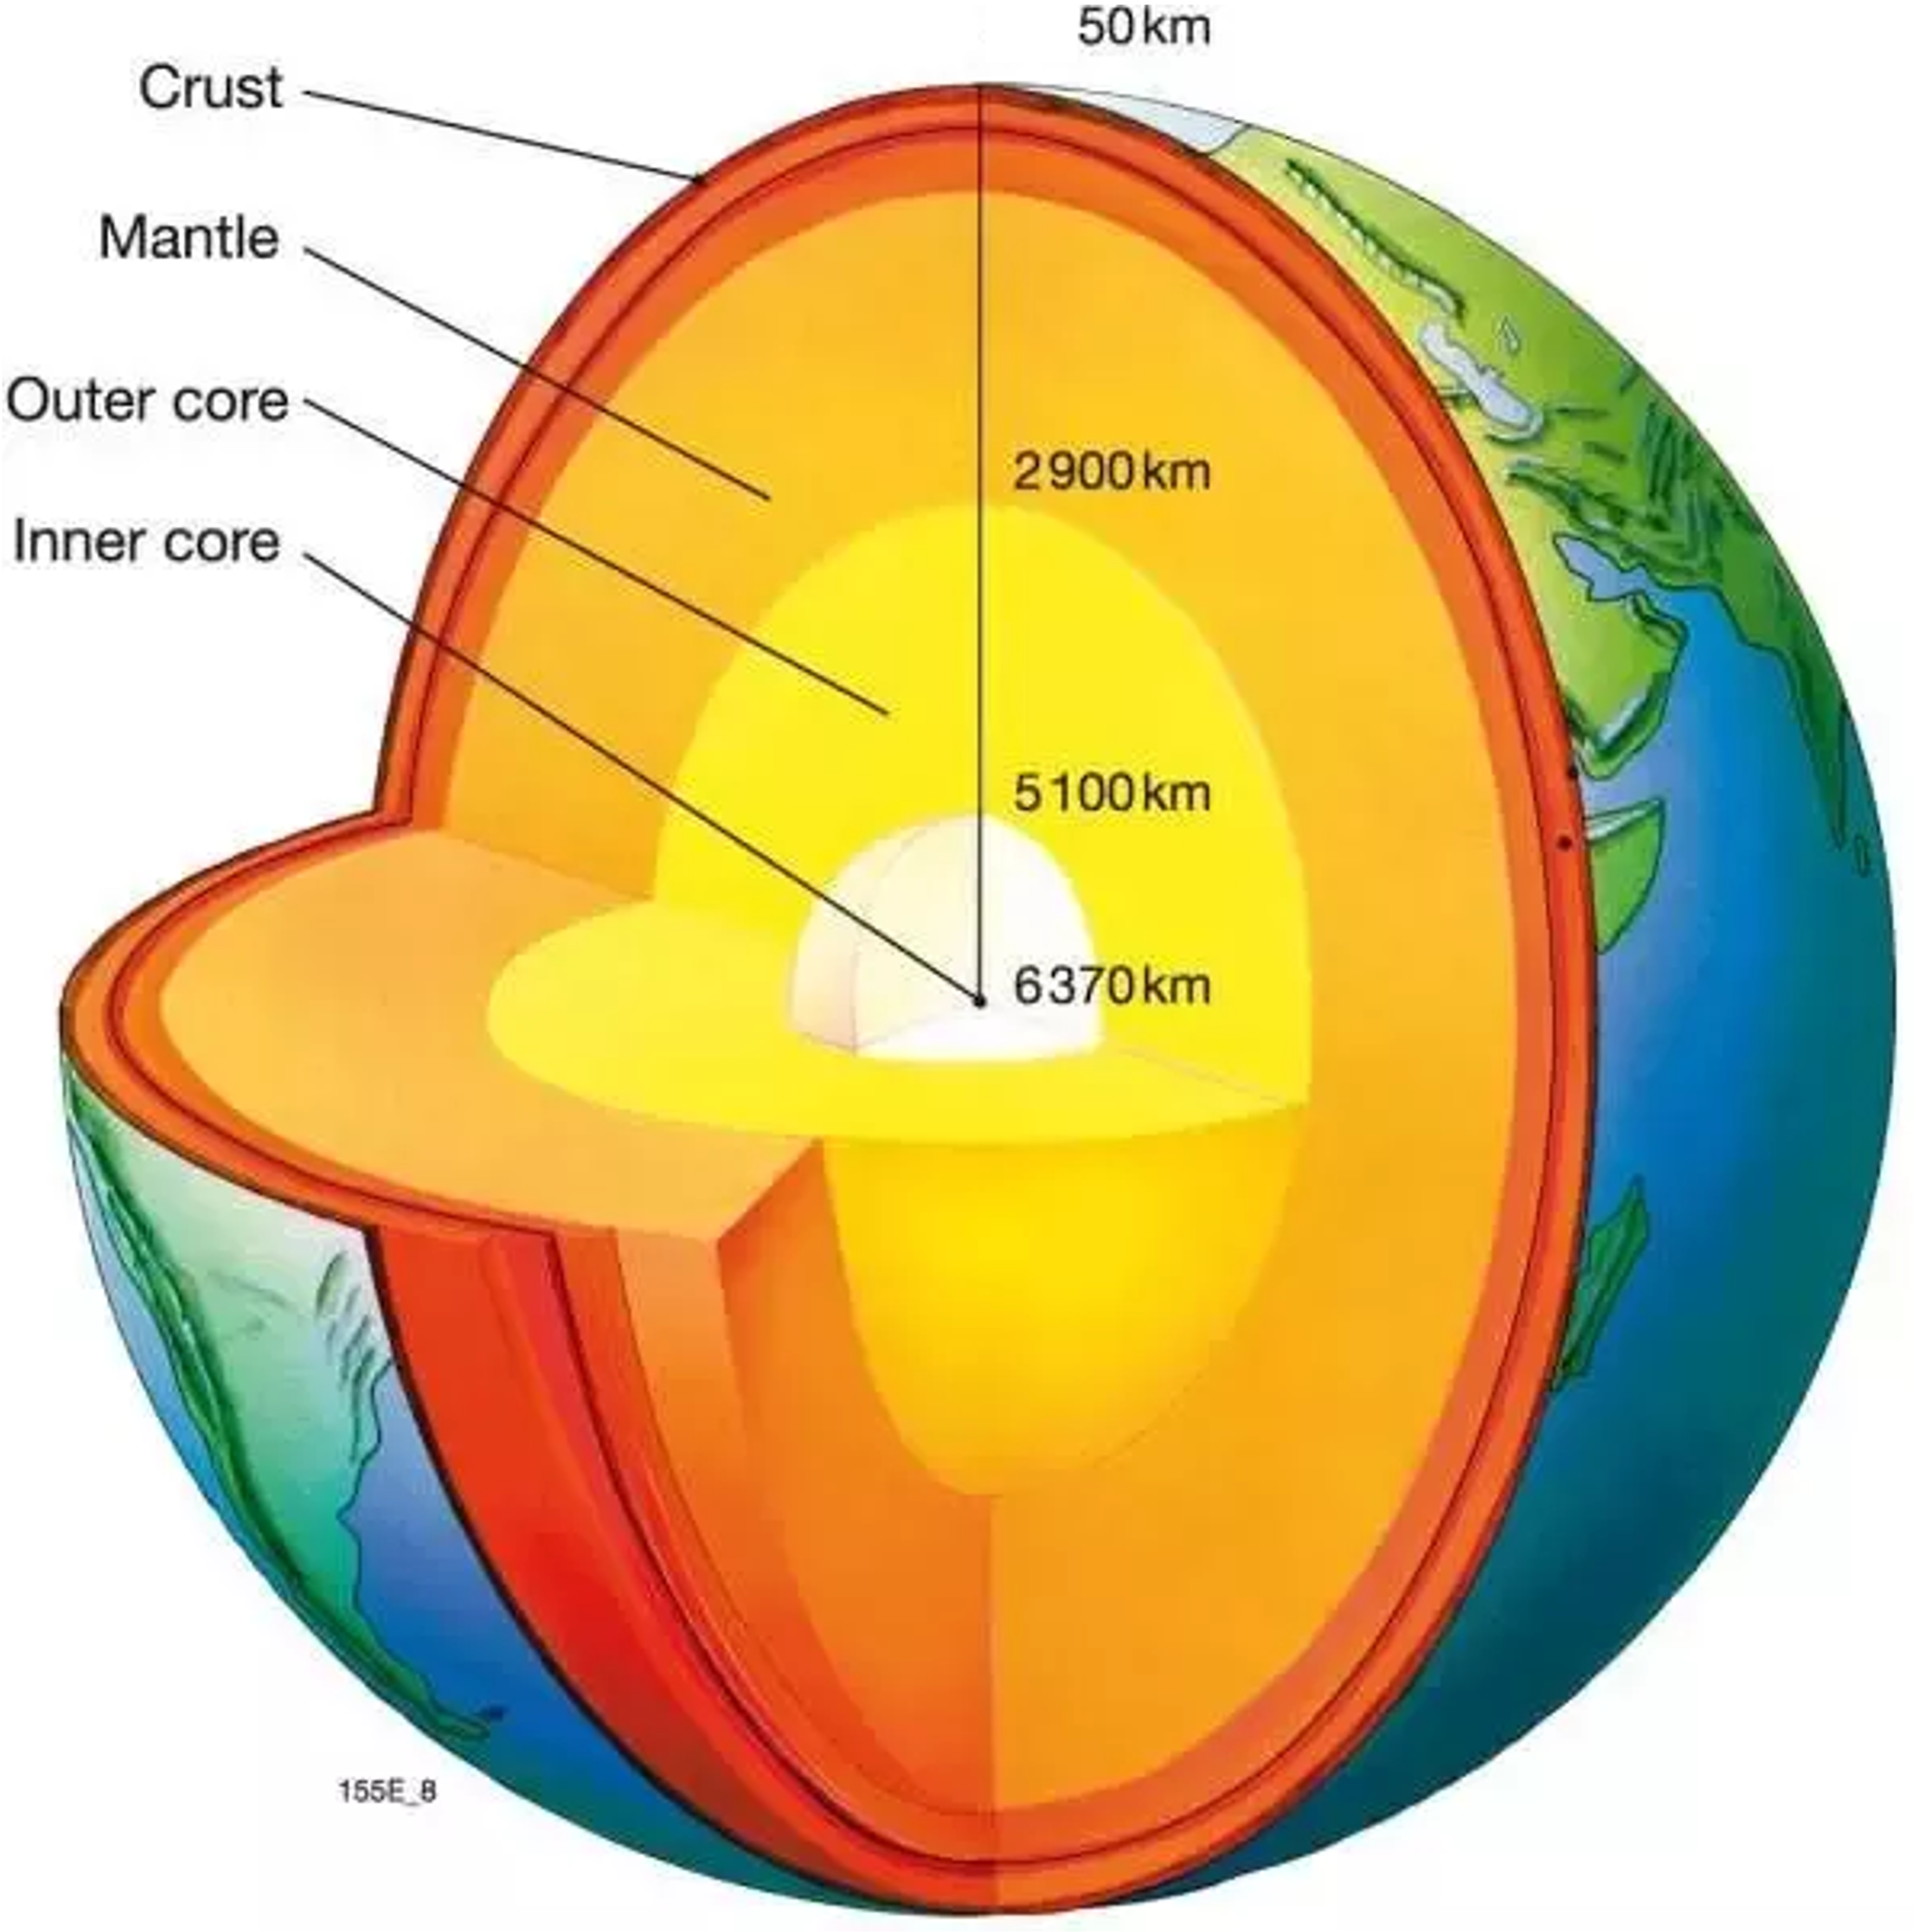
\includegraphics[height=7.5cm]{earth_layers}
        \caption{Depth from the earth's surface to the approximate maximum depth of each of the earth's layers.}
        \label{fig:earth_layers}
\end{figure}


\begin{Exercise}[title=Currency Trading]  
    
    A currency trader uses the following equation to calculate the amount in US dollars (USD) for the amount the customer pays in pounds sterling (GBP):
    $$USD = GBP \times M \times R$$
    where $R=1.38$ is the market rate and the multiplier, $M$ is found using the table below, based on the amount paid.:
    
    \begin{center}
    \begin{tabular}{ |l|c| } 
     \hline
     GBP & Multiplier  \\ 
     \hline
     $<$ 50                   & 0.9  \\ 
     $<$ 500 and \geq 50      & 0.92  \\ 
     $<$ 5,000 and \geq 500   & 0.95  \\ 
     $<$ 50,000 and \geq 5000 & 0.97  \\ 
     \geq 50,000              & 0.98  \\ 
     \hline
    \end{tabular}
    \end{center}
    
    Write a program that prints the amount in US dollars for a given amount in pounds sterling, and the effective exchange rate for the conversion= $\frac{\mbox {USD}}{\mbox {GBP}}$

\end{Exercise}

\begin{Exercise}[title=Arithmetic 

Comparison and Logical Operators] 
    Create three variables c=1.1, d=3.2, e=4.3. Create a new float variable, f, with a value of your choice. Test if f + 1.1 is:
    \begin{itemize}
        \item less than c
        \item greater than or equal to c but less than d
        \item greater than or equal to d but greater than e
        \item greater than or equal to e
    \end{itemize}
\end{Exercise}




\begin{Exercise}[title=Nested conditionals]
    \Question{Write a program that checks a number, x, and prints:
    \begin{itemize}
        \item `positive' if x is positive
        \item `negative' if x is negative
    \end{itemize}
    If x is positive the program should {\bf also} print:
    \begin{itemize}
        \item `square' if x is a square number \\(a number of the form $x = n^2$ where $n$ is an integer)
        \item  `not square' otherwise
    \end{itemize}
    }
    \Question{Write a program that:
    \begin{itemize}
        \item checks if a number is odd or even.
        \item if it is odd, checks if the number is a multiple of 3
        \item if it is even, checks if the number is a multiple of 4
    \end{itemize}

\end{Exercise}

\begin{figure}[!h]
        \centering
        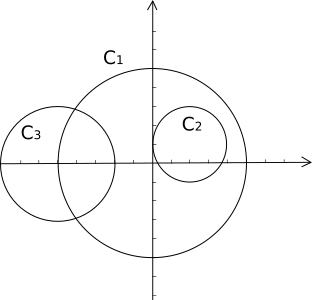
\includegraphics[height=5cm]{circles}
        \caption{Overlapping circles $C_1$, $C_2$ and $C_3$.}
        \label{fig:circles}
\end{figure}

\begin{Exercise}[title=Putting it all together: Circles] 
    
    Suppose we have three circles in the $xy$-plane (Figure \ref{fig:circles}). 
    
    Circle $C_1$ is centred at $(0, 0)$ with radius of length 5. 
    
    Circle $C_2$ is centred at $(2, 1)$ and has radius of length 2. 
    
    Circle $C_3$ is centred at $(-5, 0)$ and has a radius of length 3. 
    
    %Using conditional statements
    Write a program which takes in the variables {\tt x} and {\tt y} and tells the user which circle(s) the point $(x, y)$ is in. 
    
    Think about the order in which your program evaluates the expressions? Is this the most efficient way to structure the code? 
    
\end{Exercise}
\end{document}